\documentclass[aspectratio=169,11pt]{beamer}
\usetheme{Boadilla}
\usecolortheme{default}
\usepackage[T1]{fontenc}
\usepackage{lmodern}
\usepackage{amsmath,amssymb,mathtools,booktabs,graphicx}
\usepackage{array}
\definecolor{ink}{HTML}{202B35}
\definecolor{blue}{HTML}{246D8E}
\definecolor{rust}{HTML}{BD654B}
\setbeamercolor{normal text}{fg=ink,bg=white}
\setbeamercolor{structure}{fg=blue}
\setbeamercolor{frametitle}{fg=ink,bg=white}
\setbeamercolor{block title}{fg=white,bg=blue}
\setbeamercolor{block body}{fg=ink,bg=blue!6}
\setbeamertemplate{navigation symbols}{}
\setbeamertemplate{footline}[frame number]
\setbeamertemplate{itemize items}[circle]
\setlength{\tabcolsep}{5pt}
\newcommand{\rhos}{\rho_{S,t}}
\newcommand{\rhhat}{\widehat\rho_{S,t}}
\newcommand{\mem}{M_{\mathrm{eff}}}
\newcommand{\good}[1]{\textcolor{blue}{\textbf{#1}}}
\newcommand{\caution}[1]{\textcolor{rust}{\textbf{#1}}}
\newcommand{\src}[1]{\vfill{\tiny\color{gray}Source: #1}}
\title{Choosing memory in online copula estimation}
\subtitle{Estimators, adaptation rules, and regret\\Post-RNG-fix results}
\author{Thesis progress presentation}
\date{22 September 2026}

\begin{document}

% 1 — 0:30
\begin{frame}
  \titlepage
  \vspace{-1.0em}
  \begin{center}\small
    How should an online estimator trade statistical efficiency against adaptation
    when dependence changes?
  \end{center}
\end{frame}

% 2 — 1:00
\begin{frame}{What the estimator sees}

\[
  \underbrace{P_{i,t}}_{\text{price}}
  \;\longrightarrow\;
  \underbrace{
    X_{i,t}=\log P_{i,t}-\log P_{i,t-1}
  }_{\text{log return}}
  \;\longrightarrow\;
  \underbrace{(U_t,V_t)}_{\text{pseudo-observations}}
  \;\longrightarrow\;
  \underbrace{\widehat\rho_{S,t}}_{\text{dependence estimate}}
\]

  \begin{itemize}
    \item Returns are transformed into rolling marginal ranks,
          giving copula pseudo-observations $(U_t,V_t)$.
    \item The target is the current Spearman dependence
      \[
        \rho_{S,t}=12\,\mathbb E_{C_t}[U_tV_t]-3.
      \]
    \item The online estimator sees only data up to time $t$;
          it never observes the true $\rho_{S,t}$.
    \item In synthetic experiments, the true $\rho_{S,t}$ is retained
          only for evaluation after the estimate is made.
  \end{itemize}

  \smallskip
  \small On a real feed, truth-based RMSE and regret are therefore unavailable.

  \src{\texttt{experiments/copula\_source.hpp};
       \texttt{src/consumer/device\_state.hpp}}
\end{frame}

% 3 — 1:15
\begin{frame}{Two nonparametric representations of dependence}
  \small

  \textbf{Xiao: discounted empirical copula histogram}
  \par Pseudo-observations add mass to bins $B_{ij}$; older mass is discounted.

  \[
    N_{ij,t}
      = \lambda N_{ij,t-1}
      +(1-\lambda)\mathbf 1\{(U_t,V_t)\in B_{ij}\}.
  \]

  \[
    \widehat\rho_{S,t}
      \approx 12\sum_{ij}\widehat p_{ij,t}u_i v_j-3.
  \]

  \smallskip

  \textbf{Hermite: smooth basis representation}
  \par New observations update smooth coefficients rather than bin masses.

  \[
    A_t=(1-\alpha)A_{t-1}
        +\alpha\,h(X_t)h(Y_t)^\top,
    \qquad
    \widehat\rho_{S,t}
      =\mathcal R(A_t,\text{marginal coefficients}).
  \]

  \smallskip

  \good{Same target, different representation: Xiao stores local mass; Hermite stores smooth coefficients.}

  \src{\texttt{xiao\_spearman.hpp};
       \texttt{hermiter.hpp};
       \texttt{memory\_sweep.md}}
\end{frame}

% 4 — 1:00
\begin{frame}{Parametric arm: Gaussian-copula Fisher scoring}

  \textbf{Assume the copula is Gaussian.}
  Then dependence is described by one parameter, the correlation $r_t$.

  \medskip

  Update it online on the unconstrained scale
  $\theta_t=\operatorname{atanh}(r_t)$:
  \[
    H_t=\lambda H_{t-1}+I_\theta,
    \qquad
    \theta_t=\theta_{t-1}+\frac{s_t}{H_t}.
  \]

  \begin{itemize}
    \item $s_t$ tells us whether the new observation pushes dependence up or down.
    \item $\lambda$ controls how quickly old information is forgotten:
          larger $\lambda$ means longer memory.
  \end{itemize}

  Convert back to the common Spearman target:
  \[
    \widehat\rho_{S,t}
      =\frac{6}{\pi}\arcsin\!\left(\frac{\widehat r_t}{2}\right).
  \]

  \good{Less to estimate than Xiao or Hermite, but only if the Gaussian-family assumption is appropriate.}

  \src{\texttt{gaussian\_mle.hpp}; \texttt{memory\_sweep.md} \S9}
\end{frame}

% 5 — 1:00
\begin{frame}{Model-based arm: local-level Kalman filter}

  \textbf{Treat dependence as a hidden state that can move over time.}

  \medskip

  Every block gives a noisy Spearman estimate on Fisher's scale:
  \[
    y_b=\operatorname{atanh}(\widehat\rho_{S,b}),
    \qquad
    z_b=z_{b-1}+\omega_b,
    \qquad
    y_b=z_b+\varepsilon_b.
  \]

  The Kalman filter combines the previous estimate with the new block:
  \[
    K_b=\frac{P_b^-}{P_b^-+R},
    \qquad
    \widehat z_b
      =\widehat z_b^-+K_b\bigl(y_b-\widehat z_b^-\bigr).
  \]

  \begin{itemize}
    \item Small $K_b$: trust the past more $\Rightarrow$ longer memory.
    \item Large $K_b$: trust the new block more $\Rightarrow$ shorter memory.
  \end{itemize}

  \good{Here memory is controlled by how uncertain we think the latent dependence is.}

  \src{\texttt{kalman\_local\_level.hpp};
       \texttt{kalman\_changepoint\_results.md}}
\end{frame}

% 6 — 1:10
\begin{frame}{Exponential forgetting and fixed memory}

  \textbf{Exponential forgetting:} new observations receive more weight,
  while older observations fade geometrically.

  \[
    \alpha,\quad
    \alpha(1-\alpha),\quad
    \alpha(1-\alpha)^2,\quad
    \alpha(1-\alpha)^3,\ldots
  \]

  \[
    \alpha\uparrow
    \Rightarrow
    \text{faster forgetting}
    \Rightarrow
    \text{shorter memory}.
  \]

  With $w_j=\alpha(1-\alpha)^j$, define the weight-equivalent memory
  \[
    \mem
      =\frac{(\sum_{j\ge0}w_j)^2}{\sum_{j\ge0}w_j^2}
      =\frac{2-\alpha}{\alpha}.
  \]

  \small
  For example, $\alpha=0.1$ gives $\mem=19$.

  \medskip

  \good{Fixed memory means choosing one update rate --- equivalently one
  $\mem$ --- and keeping it unchanged for the whole run.}

  \medskip
  \scriptsize
  $\mem$ measures weight concentration; serial dependence can make the
  statistical effective sample size different.

  \src{\texttt{memory\_sweep.md} \S1, \S3;
       \texttt{study\_config.hpp}}
\end{frame}

% 7 — 1:00
\begin{frame}{How memory enters each estimator}

  \textbf{Each estimator remembers something different, but each controls
  how strongly new data can replace the past.}

  \medskip

  \begin{center}
  \small
  \begin{tabular}{lll}
    \toprule
    Estimator & What is remembered & Shorter memory when \\
    \midrule
    Xiao
      & bin masses
      & $\alpha=1-\lambda$ increases \\

    Hermite
      & basis coefficients
      & $\alpha$ increases \\

    Gaussian Fisher
      & accumulated information $H_t$
      & $1-\lambda$ increases \\

    Kalman
      & latent dependence state
      & gain $K_t$ increases \\
    \bottomrule
  \end{tabular}
  \end{center}

  \medskip

  \[
    \text{more weight on new data}
    \quad\Longrightarrow\quad
    \text{shorter memory}.
  \]

  \good{The mechanics differ, but the underlying question is the same:
  how much should new information outweigh the past?}

  \src{\texttt{xiao\_spearman.hpp};
       \texttt{hermiter.hpp};
       \texttt{gaussian\_mle.hpp};
       \texttt{kalman\_local\_level.hpp}}
\end{frame}

% 8 — 1:00
\begin{frame}{Variable forgetting factor: adapt memory using surprise}

  Fixed memory keeps the same update strength throughout the run.

  \medskip

  \textbf{VFF asks whether the new data agrees with the estimator's current state,
  then adjusts memory accordingly.}

  \medskip

  \begin{center}
  \small
  \begin{tabular}{lll}
    \toprule
    Estimator & What counts as surprise & What changes memory \\
    \midrule
    Xiao
      & $g_t-\widehat\rho_{S,t-1}$
      & $\alpha_t$ \\

    Hermite
      & coefficient-pattern change
      & $\alpha_t$ \\

    Fisher
      & score surprise
      & $\lambda_t$ \\

    Kalman
      & $e_b^2/F_b$
      & $Q_t \rightarrow K_t$ \\
    \bottomrule
  \end{tabular}
  \end{center}

  \[
    \text{large surprise}
    \Rightarrow
    \text{trust new data more}
    \Rightarrow
    \text{shorter memory},
  \]
  \[
    \text{quiet data}
    \Rightarrow
    \text{trust the past more}
    \Rightarrow
    \text{longer memory}.
  \]

  \good{Same feedback idea; different definitions of surprise and memory.}

\end{frame}

% 9 — 0:55
\begin{frame}{VFF worked example: Xiao}

  A new pseudo-observation $(U_t,V_t)$ gives the one-step dependence signal
  \[
    g_t
      =12\left(U_t-\tfrac12\right)
          \left(V_t-\tfrac12\right),
    \qquad
    \mathbb E[g_t]=\rho_{S,t}.
  \]

  Compare it with Xiao's current estimate:
  \[
    e_t=g_t-\widehat\rho_{S,t-1}.
  \]

  \begin{center}
    \emph{How surprising was the new observation relative to my
    current dependence estimate?}
  \end{center}

  Smooth the recent squared surprise:
  \[
    C_t=(1-r)C_{t-1}+r e_t^2.
  \]

  \[
    C_t\uparrow
    \Rightarrow
    \alpha_t\uparrow
    \Rightarrow
    \text{shorter memory},
    \qquad
    C_t\downarrow
    \Rightarrow
    \alpha_t\downarrow
    \Rightarrow
    \text{longer memory}.
  \]

  \good{VFF turns persistent prediction error into faster forgetting.}

  \src{\texttt{adaptive\_memory.md} \S5;
       \texttt{xiao\_spearman.hpp}}
\end{frame}

% 8 — 1:15
\begin{frame}{Bank: compete over fixed memories}
  \good{The bank is a weighted vote among fixed-memory estimators.}
  All arms see the same returns; only their memory lengths differ.
  \begin{enumerate}
    \item Each arm gives an estimate \emph{before} seeing the new pair.
    \item Score its error against the observable rank-pair signal
    $g_t=12(U_t-\tfrac12)(V_t-\tfrac12)$:
  \end{enumerate}
  \[
    \ell_{k,t}=\frac{(g_t-\widehat\rho_{k,t-1})^2}{2v_t},
    \quad v_t=\text{common predictive scale}.
  \]
  \begin{enumerate}\setcounter{enumi}{2}
    \item Every 20 ticks, give better-scoring arms more weight:
  \end{enumerate}
  \[
    \widetilde w_{k,b}\propto w_{k,b-1}
    \exp\!\left(-\eta\sum_{t\in b}\ell_{k,t}\right),\quad
    w_{k,b}=(1-\gamma)\widetilde w_{k,b}+\frac\gamma K.
  \]
  Report $\widehat\rho_b=\sum_k w_{k,b}\widehat\rho_{k,b}$.
  $\eta$ controls reaction speed; fixed share $\gamma/K$ keeps every arm available.
  \par\tiny Related to exponential expert weighting with fixed share and multiple-model estimation.
  \src{\texttt{estimator\_bank.hpp}; \texttt{adaptive\_memory.md} \S17}
\end{frame}

% 9 — 1:00
\begin{frame}{How we score: RMSE, bias, and variance}

  Run the same synthetic experiment $S$ times with different seeds.
  At tick $t$, $\widehat\rho_t^{(s)}$ is run $s$'s estimate and
  $\rho_{S,t}$ is the known truth.

  \[
    \overline{\widehat\rho}_t
      =\frac1S\sum_{s=1}^S \widehat\rho_t^{(s)}
  \]

  \[
    \operatorname{Bias}_t^2
      =(\overline{\widehat\rho}_t-\rho_{S,t})^2,
    \qquad
    \operatorname{Var}_t
      =\frac1S\sum_{s=1}^S
      (\widehat\rho_t^{(s)}-\overline{\widehat\rho}_t)^2.
  \]

  Over scoring window $W$,
  \[
    \operatorname{RMSE}_W
      =
      \sqrt{
        \frac1{|W|}
        \sum_{t\in W}
        \left(
          \operatorname{Bias}_t^2+\operatorname{Var}_t
        \right)
      }.
  \]

  \small
  \textbf{Bias:} systematic distance from truth. \qquad
  \textbf{Variance:} instability across runs.

  \medskip
  \good{Short memory is responsive but noisy; long memory is stable but can lag.}

  \src{\texttt{memory\_sweep.md} \S4;
       synthetic runs with known $\rho_{S,t}$}
\end{frame}

% 10 — 1:15
\begin{frame}{How we score: regret}
  \small
  On scoring window $W$, let
  $\ell_t(j)=(\widehat\rho_{j,t}-\rho_{S,t})^2$ and
  $L_W(j)=\sum_{t\in W}\ell_t(j)$.

  \smallskip

  \textbf{Static regret:}
  compare with the best \emph{single fixed memory} chosen in hindsight:
  \[
    R_W^{\mathrm{static}}(j)
      =
      L_W(j)
      -
      \underbrace{\min_k L_W(k)}_{\text{best one memory for the whole window}}.
  \]

  \textbf{Switching regret:}
  compare with a hindsight oracle allowed to change memory:
  \[
    R_W^{\mathrm{switch},m}(j)
      =
      L_W(j)
      -
      \underbrace{
      \min_{\#\text{ switches}\le m}
      \sum_{t\in W}\ell_t(k_t)
      }_{\text{best changing-memory sequence}}.
  \]

  \smallskip
  $R>0$: method leaves error on the table. \qquad
  $R<0$: method beats that comparator.

  \good{Static regret measures robustness to choosing one memory;
        switching regret measures how much adaptation opportunity was missed.}

  \src{\texttt{adaptive\_memory.md} \S12--\S13}
\end{frame}

% 11 — 1:00
\begin{frame}{RMSE and regret answer different questions}

  \begin{center}
  \small
  \begin{tabular}{p{0.24\textwidth} p{0.34\textwidth} p{0.34\textwidth}}
    \toprule
    & \textbf{RMSE} & \textbf{Regret} \\
    \midrule

    Question
    & How accurate is the estimator?
    & How much worse is it than the best comparator? \\[1mm]

    Reference
    & True dependence $\rho_{S,t}$
    & Best fixed or switching strategy in hindsight \\[1mm]

    What it reveals
    & Bias, variance, and overall tracking error
    & Cost of using the wrong memory or adapting too slowly \\[1mm]

    Best use
    & Comparing statistical accuracy
    & Evaluating robustness and adaptation \\

    \bottomrule
  \end{tabular}
  \end{center}

  \medskip

  \[
    \operatorname{RMSE}
    \;\approx\;
    \text{``How wrong am I?''}
    \qquad
    \operatorname{Regret}
    \;\approx\;
    \text{``How much opportunity did I miss?''}
  \]

  \good{RMSE measures estimation quality; regret measures the cost of not using
  the best memory strategy for that regime.}

\end{frame}

% 11 — 1:00
\begin{frame}{The experimental question}
  \begin{center}
  \begin{tabular}{ll}
    \toprule
    Dependence regime & What it tests\\
    \midrule
    Constant & Long-run variance\\
    Drift & Tracking a moving target\\
    Jump & Adaptation and recovery\\
    Oscillation & Repeated changes\\
    \bottomrule
  \end{tabular}
  \end{center}
  \medskip
  Compare fixed memory, VFF, and banks on the same target and scenarios.
  State the window with every RMSE or regret: the full run can conceal recovery loss.
  All results shown next use the regenerated, portable-RNG streams.
  \src{\texttt{memory\_sweep.md}; \texttt{adaptive\_memory.md}; \texttt{results\_2026\_09\_22.md}}
\end{frame}

% 12 — 1:15
\begin{frame}{Result 1: all four methods shift memory with the regime}
  \small Longer memory reduces variance but increases lag under local drift:
  \[
    \operatorname{MSE}(M)\approx
      \underbrace{\sigma^2/M}_{\text{variance}}
      +\underbrace{(dM/2)^2}_{\text{lag bias}}
    \qquad\text{(local-linear-drift heuristic).}
  \]
  \begin{center}
  \begin{tabular}{lrrrr}
    \toprule
    Window & Xiao & Hermite & Fisher & Kalman$^\dagger$\\
    \midrule
    Drift            & $341$ & $341$ & $235$ & $\sim360$\\
    Oscillation      & $36$  & $36$  & $36$  & $\sim32$\\
    Jump: whole run  & $162$ & $162$ & $162$ & $\sim148$\\
    Jump: recovery   & $53$  & $53$  & $36$  & $\sim63$\\
    Jump: settled    & $495$ & $719$ & $495$ & $\sim879$\\
    \bottomrule
  \end{tabular}
  \end{center}
  \scriptsize Entries minimise measured RMSE over each method's tested memory grid,
  in ticks, on Gaussian-copula data (40 seeds). $^\dagger$Kalman memory is an
  approximate block-to-tick conversion. Constant dependence has no stable
  interior optimum; Hermite's long-memory end is warm-up limited.
  \par\smallskip
  \small\good{The broad ordering repeats across methods: rapid change favours short
  memory; settled dependence favours longer memory.}
  \src{Post-RNG-fix \texttt{experiments/results/memory\_sweep.csv}; \texttt{memory\_sweep.md} \S3--\S6}
\end{frame}

% 13 — 1:00
\begin{frame}{Result 2: processing rate changes optimal memory}
  If only fraction $f$ of ticks is processed, $M_{\rm ticks}$ ticks contain
  $fM_{\rm ticks}$ observations. Under local linear drift $d$,
  \[
    \operatorname{MSE}(M_{\rm ticks})
      \approx\frac{\sigma^2}{fM_{\rm ticks}}
       +\left(\frac{dM_{\rm ticks}}{2}\right)^2,
    \qquad M_{\rm ticks}^*\propto f^{-1/3}.
  \]
  The measured optimum rose $1.24$--$1.29\times$ at half rate (prediction
  $1.26\times$) and $1.52$--$1.63\times$ at quarter rate (prediction $1.59\times$).
  \src{\texttt{results\_2026\_09\_22.md} \S0; post-RNG-fix linear-drift runs}
\end{frame}

\begin{frame}{Result 3: parametric gains are reliable only on-family}
  At matched memory, online Gaussian-copula Fisher scoring has two different records:
  \begin{center}
  \begin{tabular}{lcc}
    \toprule
    Data-generating family & Lower mean error than Xiao & Worst observed loss\\
    \midrule
    Gaussian (correct model) & \good{6 of 6 windows} & ---\\
    Non-Gaussian (wrong model) & 8 of 18 windows & \caution{$+55.2\%$}\\
    \bottomrule
  \end{tabular}
  \end{center}
  \medskip
  \good{Correct specification buys efficiency;} incorrect specification can erase or
  reverse it. Xiao does not assume a Gaussian copula.
  \src{\texttt{results\_2026\_09\_22.md} \S0; post-RNG-fix sweep, 40 seeds}
\end{frame}

% 14 — 1:15
\begin{frame}{Result 4: the bank reduces worst-case regret}
  Here regret is scenario mean squared loss minus the lowest mean squared loss
  among evaluated comparator strategies in that family.
  \begin{center}
  \begin{tabular}{lrrr}
    \toprule
    Family & Bank & Best fixed & Best VFF\\
    \midrule
    Xiao & \good{$2.08$} & $11.22$ & $38.49$\\
    Hermite & \good{$2.16$} & $12.83$ & $67.73$\\
    Hermite, debiased & \good{$1.90$} & $12.79$ & $67.73$\\
    Gaussian MLE & \good{$2.46$} & $9.23$ & ---\\
    Kalman & \good{$4.16$} & $18.14$ & $14.68$\\
    \bottomrule
  \end{tabular}
  \end{center}
  \small Values are worst-case regret across four scenarios, in $10^{-3}$ MSE units.
  \good{The bank cuts worst-case regret by about 73--85\% relative to the best
  fixed memory strategy} in each family.
  \src{\texttt{results\_2026\_09\_22.md} \S0; post-RNG-fix \texttt{adaptive\_memory.csv}}
\end{frame}

% 15 — 1:15
\begin{frame}{Result 5: switching reveals delayed recovery}
  Let $L^*(0)$ be the best single memory in hindsight and $L^*(1)$ the best
  sequence with one hindsight switch. Define
  \[
    \mathrm{capture}=
    \frac{L^*(0)-L_{\mathrm{bank}}}{L^*(0)-L^*(1)}.
  \]
  \begin{center}
  \begin{tabular}{lrr}
    \toprule
    Bank family & One-switch capture & Interpretation\\
    \midrule
    Xiao & $5.6\%$ & Most switch value missed\\
    Hermite, debiased & $6.9\%$ & Most switch value missed\\
    Gaussian MLE & $3.3\%$ & Most switch value missed\\
    Kalman & \good{$73.3\%$} & Captures much more switch value\\
    \bottomrule
  \end{tabular}
  \end{center}
  The hindsight oracle switches among continuously running arms; it does not reset them.
  \src{\texttt{results\_2026\_09\_22.md} \S0; post-RNG-fix, full synthetic jump run}
\end{frame}

% 16 — 1:15
\begin{frame}{Result 6: where the bank's whole-run advantage comes from}
  Xiao-bank excess squared loss against the best fixed Xiao memory:
  \begin{center}
  \begin{tabular}{lrrr}
    \toprule
    Before jump & Recovery & Settled & Whole run\\
    \midrule
    \good{$-7{,}727$} & \caution{$+5{,}902$} & $+1{,}076$ & $-749$\\
    \bottomrule
  \end{tabular}
  \end{center}
  \medskip
  \small One fixed-memory comparator is chosen over the whole run and held fixed in
  every window. Negative means the bank is ahead. It earns its advantage before the jump,
  then gives much of it back during recovery. Raising $\eta$ improves recovery
  but damages worst-case regret on oscillation.
  \medskip
  \small Units: cumulative squared loss $\times10^{-3}$; window boundaries are
  those of the offline jump protocol.
  \src{\texttt{results\_2026\_09\_22.md} \S0; post-RNG-fix \texttt{switching\_loss.csv}}
\end{frame}

% 17 — 1:00


\begin{frame}{What changed, and how memory responded}
  \begin{center}
    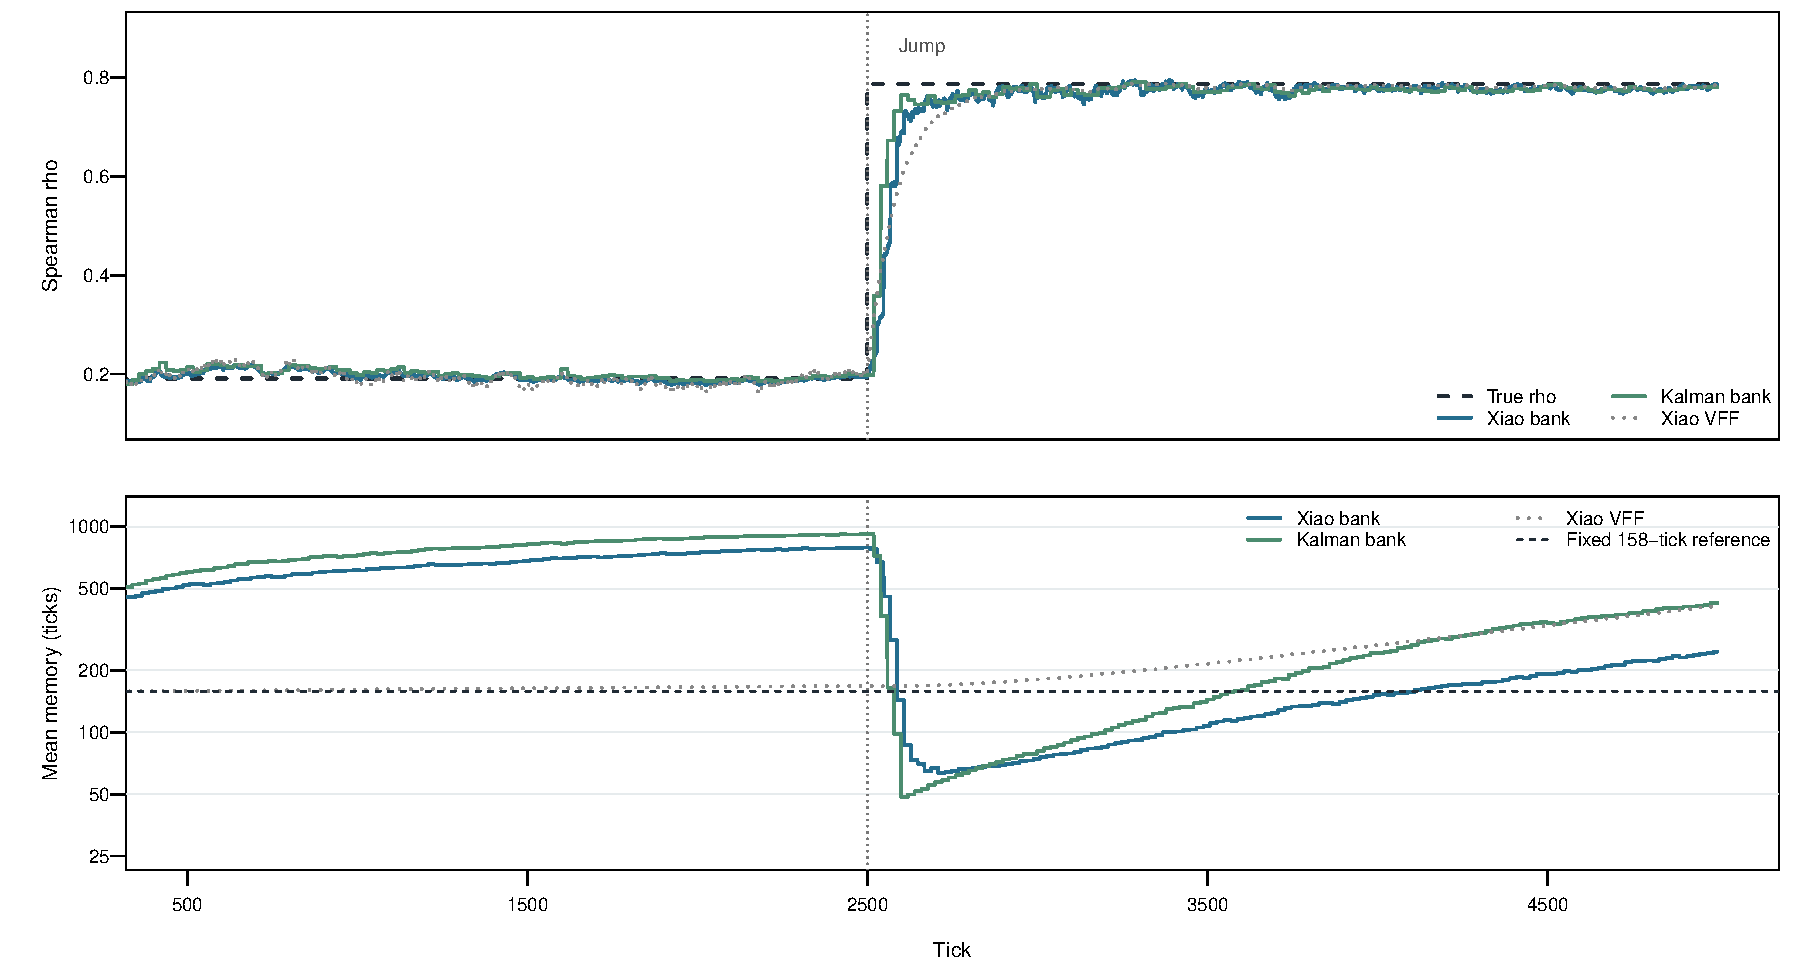
\includegraphics[width=0.71\linewidth]{copula-memory-beamer/figures/dependence_and_memory_post_rng.pdf}
  \end{center}
  \vspace{-0.2cm}
  \small Top: true $\rho_S$ jumps from 0.19 to 0.79; estimates catch up.
  Bottom: $\bar M_b=\sum_k w_{k,b}M_k$ falls as weight shifts from long to short arms.
  \good{The memory drop is reweighting, not a reset.}
  \src{\texttt{adaptive\_memory\_traj.csv}; post-RNG-fix runs}
\end{frame}

% 18 — 0:45
\begin{frame}{Streaming validation: mechanism reproduced}
  Simulated prices traversed producer $\to$ broker $\to$ consumer, then log-price
  differences fed eight estimators.
  \begin{itemize}
    \item A seeded source and pair IDs make the stream reproducible and alignable.
    \item In the controlled jump run, there were no missing or unmatched pairs after
          connection; the recorded change occurred at the configured pair ID.
    \item Fixed-memory controls stayed flat; bank memory shortened around the jump.
  \end{itemize}
  \begin{block}{What this establishes}
    Transport and qualitative adaptation, not a performance gain. Same-input
    live/probe estimator parity and a replicated scoring study remain to be done.
  \end{block}
  \src{\texttt{online\_run\_2026\_09\_22.md}; commit \texttt{479ebdc}; \texttt{rng\_portability.md}}
\end{frame}

% 19 — 0:30
\begin{frame}{Three findings to take away}
  \begin{enumerate}
    \item \good{Preferred memory is similar across Xiao and Gaussian Fisher scoring.}\par\smallskip
      Xiao and the Gaussian MLE agree within one memory-grid step in 21 of 24 cells;
      exact agreement occurs in 13.
    \medskip
    \item \good{The bank has the lowest tested worst-case regret.}\par\smallskip
      Its worst-case regret is about 73--85\% below the best fixed memory
      strategy across five estimator families.
    \medskip
    \item \caution{A whole-run gain does not imply fast recovery.}\par\smallskip
      The Xiao bank gains before the jump and loses ground immediately after it.
  \end{enumerate}
  \medskip
  \small A controlled seeded stream reproduces the mechanism; same-input estimator
  parity and replicated scoring are still needed for performance claims on that path.
\end{frame}



\appendix
\begin{frame}{Backup: native controls on the common memory scale}
  \begin{center}
  \begin{tabular}{lll}
    \toprule
    Method & Code parameter & Approximate update weight $\alpha$\\
    \midrule
    Xiao histogram & retention $\lambda$ & $1-\lambda$\\
    Hermite expansion & update weight $\lambda$ & $\lambda$\\
    Gaussian Fisher scoring & information retention $\lambda$ & $1-\lambda$\\
    Kalman filter & gain $K$ per $m$-tick block & $\mem\simeq m(2-K)/K$\\
    \bottomrule
  \end{tabular}
  \end{center}
  \src{\texttt{memory\_sweep.md} \S1, \S3; \texttt{study\_config.hpp}}
\end{frame}

\end{document}
